\documentclass[letterpaper, 10 pt, conference]{ieeeconf}  % Comment this line out
                                                          % if you need a4paper
%\documentclass[a4paper, 10pt, conference]{ieeeconf}      % Use this line for a4
                                                          % paper

\IEEEoverridecommandlockouts                              % This command is only
                                                          % needed if you want to
                                                          % use the \thanks command
\overrideIEEEmargins

\usepackage{graphicx}
\usepackage{lipsum}  
\usepackage{xcolor}
\usepackage{titlesec}

\titleformat{\subsection}
{\color{blue}\normalfont\itshape}
{\color{blue}\thesubsection}{1em}{}

\newif\ifsubtitles
\subtitlestrue

\newcommand{\subtitle}[1]{{
    \ifsubtitles
      \\ \small \normalfont \color{purple} #1%
    \fi
}}


\graphicspath{ {images/} }

\title{\LARGE \bf
NeuLaw's Criminal Record Database\footnote{The same datasets is also known as the Center for Science and Law’s Criminal Record Database} \\{\color{blue}Datasheet}
}

\begin{document}


\maketitle
\thispagestyle{empty}
\pagestyle{empty}

%%%%%%%%%%%%%%%%%%%%%%%%%%%%%%%%%%%%%%%%%%%%%%%%%%%%%%%%%%%%%%%%%%%%%%%%%%%%%%%%
\section{Motivation}

\subsection{For what purpose was the dataset created?}

According to the creators of the dataset, the dataset was created ``To allow large-scale, cross-jurisdictional analyses of criminal arrests" and ''enhance many types of research -- for example, identification of high-frequency offenders, measurement of changes in policing strategies, and quantification of legislative efficacy -- giving policy makers the best data upon which to base law enforcement decisions'' \cite{ormachea2015new}.

\subsection{Who created the dataset? \subtitle{Is it an official law enforcement or government body? An academic research team? Other?}}

The codebook lists Gabe Haarsma, Sasha Davenport, Pablo A. Ormachea & David M. Eagleman as authors \cite{Neulaw}.


\subsection{Was there a specific task in mind, or gap that needed to be filled?}

The dataset was created to improve on the information available from the UCR SRS program. Specifically, according to the creators, the advantages of this novel dataset include: (1) individual identifiers allow for recidivism analysis—albeit only for repeated bookings within the same
jurisdiction (2) the presence of all the charges allows
for deeper understanding of all crime, not just a subset,
(3) more and different offender-specific variables than
the UCR, (4) the data represent a comprehensive and
growing picture of information available to judges and
prosecutors, and (5) more and different disposition-specific
variables, enabling assessment of small variations in
punishment \cite{ormachea2015new}.

\subsection{Any other comments?}

There maybe an updated version of this dataset that is not freely available, from here:
href{http://scilaw.org/risk-assessment/
}{http://scilaw.org/risk-assessment/}.

\section{Composition}

\subsection{What do the instances that comprise the dataset represent? \subtitle{For example: crimes, offenders, court cases, police officers}}

Records of criminal charges. The specific variables varies depending on the jurisdiction as described below.

\subsection{Are there multiple types of instances? \subtitle{For example: offenders, victims, and the relationship between them.}}

Not within each jurisdiction.

\subsection{How many instances are there in total? \subtitle{Of each type, if appropriate.}}

\textbf{Harris County, TX:} 3.1 million records, spanning from 1977 to April, 2012. \\
\textbf{New York City, NY:} 9.8 million records spanning from 1977 to 2013. \\

\textbf{Miami-Dade County, FL:} 5.7 million records spanning from 1971 to 2012.

\subsection{Does the dataset contain all possible instances or is it a sample (not necessarily random) of instances from a larger set? \subtitle{For example, if it is traffic stops from a territory, is it all traffic stops conducted within that territory within a specific time? If not, is it a representative sample of all stops? Describe how representativeness was validated/verified. If it is not representative, please describe why.}}

The dataset includes all records from each jurisdiction, within the stated time frame. Some data instances were removed in pre-processing. In addition: 

(1) The database contains no juvenile records, as those
are not included in basic Freedom of Information Act
requests. We note that juvenile is defined differently in
each locale, so 17 year olds are included in Harris
County records whereas only 18 year olds appear in
New York City and Miami-Dade County records. \\

(2) The database does not include sealed or expunged
records, as those are typically removed from the
underlying county databases. It is likely that this
disproportionately affects certain crime types (e.g.,
traffic offenses).

\subsection{What data does each instance consist of? \subtitle{If there is a large number of variables, please provide a broad description of what is included.}}

In the \textbf{Harris County dataset}, each instance contains Information regarding the: \\
1. Offense: date, code, name, degree, bond amount at the time of arrest, category, broad category. \\
2. Defendant: unique ID, race, gender, DOB (mm/yyyy), height, weight, citizenship status. \\
3. Case: unique case ID, date filed, offense degree, case bond, case status. \\
4. Attorney: hired or assigned.
5. Grand jury: date, defendant present, and jury action code. \\
6. Disposition: date, plea, disposition (e.g., dismissed). \\


In the \textbf{New York City dataset}, each instance contains Information regarding the: \\
1. Offense: month, year. \\
2. Arrest: county, month, year, charge, crime category, broad crime category. \\
3. Defendant: race, gender, age at arrest. \\
3. Disposition: county, month, year, charge, disposition. \\

In the \textbf{Miami-Dade County dataset}, each instance contains Information regarding the: \\ 
1. Arrest: date, code, crime category, broad crime category. \\
2. Case: date filed, date closed, offense degree, trial type (Bench / Jury), case code, case status. \\
3. Defendant: race, gender, DOB (mm/yyyy). \\
4. Disposition: code, plea, disposition. 

\subsection{Is there a target label or associated with each instance? \subtitle{Please include labels that are likely to be used as target labels, e.g. recidivism.}}

There is not a pre-specified target label. However, disposition is most suitable to be used as a target label. 

\subsection{Are there recommended data splits (e.g., training, development/validation, testing)? \subtitle{If so, please provide a description of these splits, explaining the rationale behind them.}}

No.

\subsection{Does the dataset contain data on race and ethnicity? \subtitle{If so, is it based on the individual's self-description, or based on officer's impression? Was it collected or derived in post-processing? For example, by name analysis.}}

Yes. For race, this originates from the raw data and it is not clear whether it is based on the individual's self-description. 

The jurisdictions within the datasets do not identify offenders of Hispanic descent. To obtain a better understanding of the demographics, the creators have estimated the Hispanic population by last name \cite{ormachea2015new}.

\subsection{Are there any known errors, sources of noise, bias or missing data, or variables collected for only part of the datasets? \subtitle{If so, please provide a description.}}

All the records in the database were originally
entered by humans. The creators attempted to fix typographical errors. However, a larger problem is missing data. For example, some fields have become more populated with time. Birth date was not as commonly entered in some of the earlier records from the 1970s and 1980s, but becomes more rigorously entered with time 6 \cite{ormachea2015new}. 


The dataset does not contain corrections records, as most states do not consider those public. Therefore, while we know each offender’s sentence at the end of trial or plea bargaining, we cannot know how long an
offender actually served \cite{ormachea2015new}.

\subsection{Does the dataset contain data on criminal history or other data that might be considered confidential or sensitive in any way? \subtitle{For example: sexual orientations, religious beliefs, political opinions or union memberships, or locations; financial or health data; biometric or genetic data; forms of government identification, such as social security numbers; If so, please provide a description.}}

The dataset contains partial information on criminal offending, as well as demographic information. The partial criminal offending can be constructed as the dataset contains unique identification numbers that can be linked across multiple offenses in an area. For example, in Harris County, Texas, 44\% of the 1.2M uniquely identified offenders have multiple offenses -- and therefore a partial record of offense (see Figure \ref{fig:offense_dist}).

\begin{figure}[h]
    \centering
    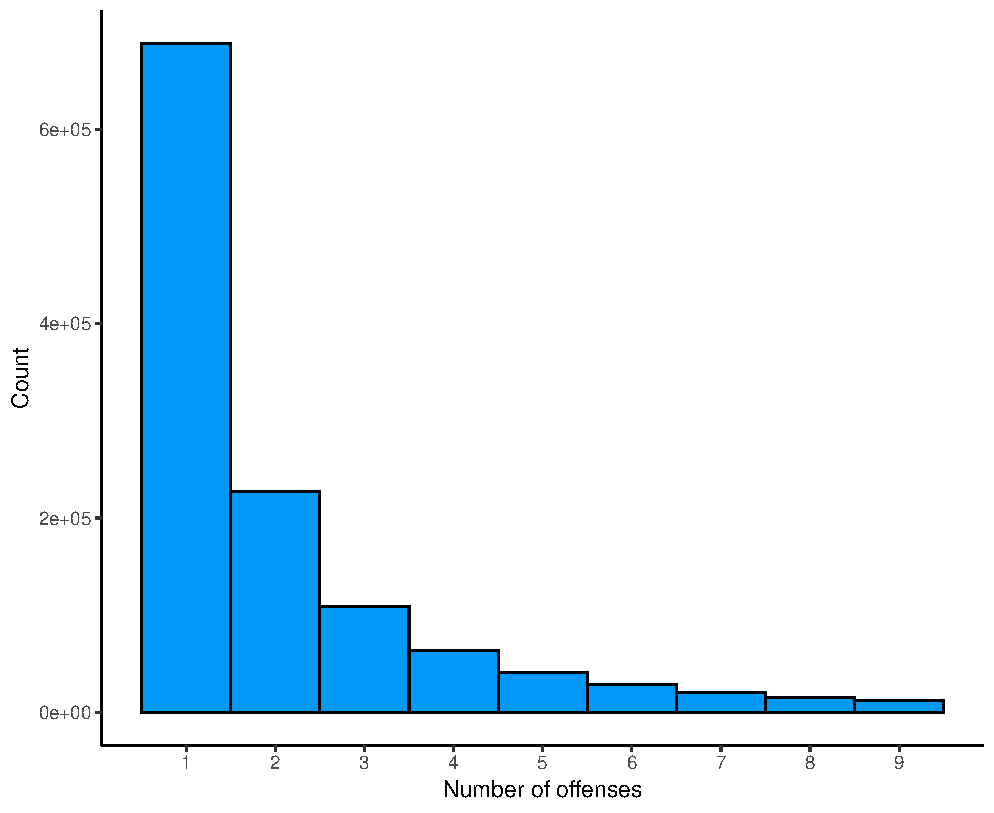
\includegraphics[width=0.5\textwidth]{Datasheets/neulaw_images/neulaw_uid.pdf}
    \caption{A histogram of the number of offenses per offender in Harris County, Texas. The visualization has been limited to offenders that have less than 10 offenses for conciseness. Individuals with more than 10 offenses represent less than 3\% of the dataset.}
    \label{fig:offense_dist}
\end{figure}

\subsection{Is it possible to identify individuals (i.e., one or more natural persons), either directly or indirectly (i.e., in combination with other data) from the dataset? \subtitle{If so, please describe how.}}

Possibly, if comparing to other sources such as news articles. Only relevant for cases that attracted media attention. 

\section{Uses}

\subsection{What type of tasks, if any, has the dataset been used for? \subtitle{If so, please provide examples and include citations.}}

Examples of papers that have used this dataset are \cite{ormachea2016enabling,bouffard2019time,cooper2018difference,pfeffer2018gendered}.


\subsection{Is there a repository that links to any or all papers or systems that use the dataset?}

No.

\subsection{What (other) tasks could the dataset be used for? \subtitle{For example: testing predictive policing systems, predicting recidivism.}}

The dataset can be used for research questions around case disposition and sentencing. A partial criminal record can be constructed from the Harris County dataset. 

\subsection{Is there anything about the composition of the dataset or the way it was collected and preprocessed/cleaned/labeled that might impact future uses? \subtitle{For example, is there anything that a dataset consumer might need to know to avoid uses that could result in unfair treatment of individuals or groups (e.g., stereotyping, quality of service issues) or other risks or harms (e.g., legal risks, financial harms)? If so, please provide a description. Is there anything a dataset consumer could do to mitigate these risks or harms?}}

The dataset only contains arrest data and not incident-based data, thus providing a picture of crime at the courthouse level. This means that previous stages in the law enforcement process (e.g., 911 calls, house calls, etc.) could skew the arrests that make it into courthouse databases  \cite{ormachea2015new}. 


The recidivism analysis allowed by this only applies for repeated bookings within the same jurisdiction. This approach will systematically undercount the true recidivism rate due to relocation  \cite{ormachea2015new}.


The dataset does not have victim data, precluding the analysis of, for example, whether ethnicity or age of victim affects sentencing  \cite{ormachea2015new}.


Some jurisdictions have more limited data than the rest. For example, New York City’s records only list the most serious offense per arrest and do not yet include an identifier \cite{ormachea2015new}. 

While our Broad categorization allows for comparisons across jurisdictions, the detailed categorization does not. The subcategories become populated only if the jurisdictions’ labels or code
citations provided enough detail \cite{ormachea2015new}.

\section{Collection Process}

\subsection{How was the data associated with each instance acquired? \subtitle {e.g. the data collected survey, the raw data is routinely collected by the courts.}}

To acquire the underlying data, the dataset creators ``contacted New York
City (New York), Harris County (Houston), and MiamiDade County (Miami), to obtain copies of their criminal records from their justice information management systems. As public records, the data were obtained via Freedom of Information Act requests'' \cite{ormachea2015new}.

\subsection{Was the information self-reported? \subtitle{If the data was self-reported, was the data validated/verified? If so, please describe how.}}

No. The data was derived from a dataset of criminal records used by respective local authorities. It was not collected for research purposes. 


\subsection{Who was involved in the data collection process? \subtitle{Was this done as part of their other duties? If not, were they compensated?}}

The data was entered into the courts data systems by employs of the courts. 

\subsection{Over what timeframe was the data collected? Does this timeframe match the creation timeframe of the data associated with the instances (e.g., recent crawl of old news articles)? \subtitle{If not, please describe the timeframe in which the data associated with the instances was created. If the collection was not continuous within the timeframe, please specify the intervals, for example, annually, every 4 years, irregularly.}}

Harris County, TX -- 1977 to April, 2012. \\
New York City, NY -- 1977 to 2013. \\
Miami-Dade County, FL -- 1971 to 2012. \\

\subsection{Were any ethical review processes conducted (e.g., by an institutional review board)? \subtitle{If so, please provide a description of these review processes, including the outcomes, as well as a link or other access point to any supporting documentation.}}


Unknown. The dataset creators do state that ``The Institutional Review
Board at Baylor College of Medicine exempted this release of an anonymized dataset from human subject research oversight because they consist of publicly available records'' \cite{ormachea2015new}.

\subsection{Were the individuals in question notified about the data collection? Did they give their consent? \subtitle{If consent was obtained, were the consenting individuals provided with a mechanism to revoke their consent in the future or for certain uses?}}

It is likely the individuals know of their criminal charges. It is unlikely they knew or gave consent for it to be used as part of a research dataset. 

\subsection{Has an analysis of the potential impact of the dataset and its use on data subjects (e.g., a data protection impact analysis) been conducted? \subtitle{If so, please provide a description of this analysis, including the outcomes, as well as a link or other access point to any supporting documentation.}}

Unknown. 

\section{Pre-processing, cleaning, labeling}

\subsection{Was any preprocessing/cleaning/labeling of the data done (e.g., discretization or bucketing, removal of instances, processing of missing values)? \subtitle{If so, please provide a description and reference to the documentation. If not, you may skip the remaining questions in this section.}}

Yes. Data processing is described is detail in \cite{ormachea2015new} and in the codebook \cite{Neulaw}. Broadly, the data was cleaned and standardized, and duplicated entries were removed. Entries have been de-identified by removing names, addresses, etc. DOB was replaced with the month and year only. In the Harris County dataset, defendants and cases were given a unique identifiers. The creators added seven calculated variables for all the datasets: 
1. Broad crime category (32 categories), 
2. Detailed crime category ($\sim 150-175$ categories)
3. Standardized disposition\footnote{standardized disposition has 7 possible dispositions: No Action, Dismissal, Transfer, Acquittal, Guilty, Guilty by Plea, Conditional Dismissal, and Unknown/No Final Disposition}
4. Gender, using given name to determine gender when missing or unknown.
5. Race, using surname to add Hispanic ethnicity.
6. The defendant age at the time of case filed or the arrest date.
7. The year the case is filed.
8. Aggregated case numbers to combine multiple offenses into single case (Harris County only).

\subsection{Was the “raw” data saved in addition to the preprocessed/cleaned/labeled data? \subtitle{If so, please provide a link or other access point to the “raw” data. }}

Yes. The calculated age, race and gender variables are added to the dataset alongside the raw variables. 

\subsection{Is the software that was used to preprocess/clean/label the data available? \subtitle{If so, please provide a link or other access point.}}

No.

\section{Distribution}


\subsection{Is the data publicly available? How and where can it be accessed (e.g., website, GitHub)? \subtitle{Does the dataset have a digital object identifier (DOI)?}}

Yes. The dataset can be found here \cite{Neulaw}.

\subsection{Is the dataset be distributed under a copyright or other intellectual property (IP) license, and/or under applicable terms of use (ToU)? \subtitle{If so, please describe this license and/or ToU, and provide a link or other access point to, or otherwise reproduce, any relevant licensing terms or ToU, as well as any fees associated with these restrictions.}}

The dataset is licensed under a Creative Commons Attribution 4.0 International (CC BY 4.0) License.

\section{Maintenance}


\subsection{Is the dataset maintained? Who is supporting/hosting/maintaining the dataset?}

The dataset is not maintained. There maybe an updated version of this dataset that is not freely available, from here:
href{http://scilaw.org/risk-assessment/
}{http://scilaw.org/risk-assessment/}.

\subsection{How can the owner/curator/manager of the dataset be contacted (e.g., email address)?}

Unknown.

\subsection{Will the dataset be updated (e.g., to correct labeling errors, add new instances, delete instances)?}

No.

\subsection{Are older versions of the dataset continue to be supported/hosted/maintained?}

N/A.

\subsection{If others want to extend/augment/build on/contribute to the dataset, is there a mechanism for them to do so? \subtitle{If so, please provide a description.}}

No.


\medskip
 
\bibliographystyle{IEEEtran}  
\bibliography{Neulaw_datasheet}

\end{document}
The owners can be contacted at: UCR-NIBRS@fbi.gov